\documentclass[12pt,a4paper,titlepage,headinclude,bibtotoc]{scrartcl}

%---- Allgemeine Layout Einstellungen ------------------------------------------

% Für Kopf und Fußzeilen, siehe auch KOMA-Skript Doku
\usepackage[komastyle]{scrpage2}
\pagestyle{plain}
\setheadsepline{0.5pt}[\color{black}]
\automark[section]{chapter}


%Einstellungen für Figuren- und Tabellenbeschriftungen
\setkomafont{captionlabel}{\sffamily\bfseries}
\setcapindent{0em}


%---- Weitere Pakete -----------------------------------------------------------
% Die Pakete sind alle in der TeX Live Distribution enthalten. Wichtige Adressen
% www.ctan.org, www.dante.de

% Sprachunterstützung
\usepackage[ngerman]{babel}

% Benutzung von Umlauten direkt im Text
% entweder "latin1" oder "utf8"
\usepackage[utf8]{inputenc}

% Pakete mit Mathesymbolen und zur Beseitigung von Schwächen der Mathe-Umgebung
\usepackage{latexsym,exscale,stmaryrd,amssymb,amsmath}


\usepackage[nointegrals]{wasysym}
\usepackage{eurosym}

% Anderes Literaturverzeichnisformat
%\usepackage[square,sort&compress]{natbib}
\usepackage{hyperref}
% Für Farbe
\usepackage{color}
\usepackage{graphicx}
\usepackage{wrapfig}
\usepackage{subfigure}

% Caption neben Abbildung
\usepackage{sidecap}

% Befehl für "Entspricht"-Zeichen
\newcommand{\corresponds}{\ensuremath{\mathrel{\widehat{=}}}}
% Befehl für Errorfunction
\newcommand{\erf}[1]{\text{ erf}\ensuremath{\left( #1 \right)}}

%Fußnoten zwingend auf diese Seite setzen
\interfootnotelinepenalty=1000

%Für chemische Formeln (von www.dante.de)
%% Anpassung an LaTeX(2e) von Bernd Raichle
\makeatletter
\DeclareRobustCommand{\chemical}[1]{%
  {\(\m@th
   \edef\resetfontdimens{\noexpand\)%
       \fontdimen16\textfont2=\the\fontdimen16\textfont2
       \fontdimen17\textfont2=\the\fontdimen17\textfont2\relax}%
   \fontdimen16\textfont2=2.7pt \fontdimen17\textfont2=2.7pt
   \mathrm{#1}%
   \resetfontdimens}}
\makeatother

%Honecker-Kasten mit $$\shadowbox{$xxxx$}$$
\usepackage{fancybox}

%SI-Package
\usepackage{siunitx}

%keine Einrückung, wenn Latex doppelte Leerzeile
\parindent0pt

%Bibliography \bibliography{literatur} und \cite{gerthsen}
%\usepackage{cite}
\usepackage{babelbib}
\selectbiblanguage{ngerman}

\begin{document}

\begin{titlepage}
\centering
%\textsc{\Large Praktikum zur Einführung in die physikalische Chemie,\\[1.5ex] Universität Göttingen}

\vspace*{3cm}

\rule{\textwidth}{1pt}\\[0.5cm]
{\huge \bfseries
  V1: Bestimmung\\[1.5ex]
  der Loschmidt-Zahl}\\[0.5cm]
\rule{\textwidth}{1pt}

\vspace*{3cm}


\begin{Large}
\begin{tabular}{ll}
Durchführende: &  Alea Tokita, Julia Stachowiak\\
Assistentin: & Annemarie Kehl\\
 Versuchsdatum: & 09.11.2015\\
 Datum der Abgabe: & 16.11.2015\\
\end{tabular}
\end{Large}

\vspace*{2.5cm}

\begin{Large}
\fbox{
  \begin{minipage}[t][2cm][t]{6cm} 
   Werte:\\
   $\Delta \lambda = 676 \pm 52 \mathrm {nm} $\\
   $ d \quad = 72 \pm 3 \mathrm{\mu m} $\\
  \end{minipage}
}
\end{Large}

\end{titlepage}

\tableofcontents

\newpage

\section{Theoretische Grundlagen}
\subsection{Stoffmenge}
Im Umgang mit chemischen Reaktionen müssen Stoffmengen betrachtet werden. Da jedoch die Teilchen, mit denen sich auseinandergesetzt wird so klein sind, ist es höchst unpraktisch mit den jeweiligen Teilchen Zahlen zu rechnen. Daher wurde die Einheit Mol eingeführt, in welcher die Stoffmenge angegeben wird. Diese Einheit ist so definiert, dass $ \mathrm{1 mol}$ einer beliebigen Substanz dieselbe Anzahl von Teilchen (Moleküle, Atome, Ionen) enthält, wie die in $\mathrm{12g}$ des Kohlenstoff-Isotops $\mathrm{^{12}C}$ enthalten sind. Diese Zahl an Teilchen, die in einem Mol enthalten sind, wird durch die Loschmidt-Zahl $N_{A}$ (oder auch Avogadro-Konstante oder Avogadro-Zahl) angegeben:\\

\begin{center}
$N_{A}=6,02214129(27)\cdot 10^{23}\mathrm{mol^{-1}}$ 
\end{center}

Mit dieser Zahl lässt sich nun die Molmasse \textit{M} einer Substanz angeben, welche die Masse eines Mols einer Sunstanz in der Einheit $ \mathrm{g \cdot mol^{-1}}$ ist. Analog bezeichnet das Molvolumen $V_{m}$ das Volumen, welches von einem Mol eines Stoffes eingenommen wird. Dieses Volumen ist temperatur- und druckabhängig.

\subsection{Elementarzelle}
In einem Kristall sind Teilchen (Atome, Ionen, Moleküle) in symmetrischer und geordneter Weise in einem sich periodisch wiederholenden, dreidimensionalen Muster angeordnet. Diese Symmetrie eines Kristalls kann mithilfe eines Kristallgitters beschrieben werden. Indem die Mittelpunkte der Teilchen gedanklich durch Gitterpunkte ersetzt werden, lässt sich aus einer Kristallstruktur ein Kristallgitter ableiten.\\
Ein Kristallgitter kann in lauter identische Elementarzellen zerlegt werden. Das Gitter ist also aus wiederholt in alle Raumrichtungen aneinandergereihte Elementarzellen aufgebaut. Dies lässt sich wieder auf die Kristallstruktur übertragen: Da der Kristall durch wiederholtes aneinanderlegen der Elementarzellen aufgebaut ist, muss die chemische Zusammensetzung einer Elementarzelle exakt der Zusammensetzung der Substanz entsprechen\footnote{Vgl. Mortimer, S. 180}.\\\\
Je nach ihrer Symmetrie können Kristallgitter in Gittertypen eingeteilt werden, die sich in der Metrik ihrer Elementarzellen unterscheiden\footnote{ebd.}. Mithilfe von Röntgenstrahlung bekannter Wellenlänge kann die Strukur und Größe einer Elementarzelle, also ihre Gitterstruktur und Gitterkonstante \textit{a} bestimmt werden. Hier einige Beispiele solcher Messungen, es sind die von uns zu vermessenden Kristalle:\\\\


\begin{figure} [h]
\begin{center}
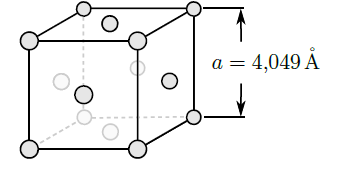
\includegraphics[scale=0.7]{Aluminium.png} \end{center}
\caption{Kristallstruktur von Aluminium$^a$}
\end{figure}

\begin{figure} [h]
\begin{center}
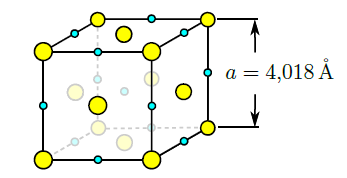
\includegraphics[scale=0.7]{Lithiumflourid.png} \end{center}
\caption{Kristallstruktur von Lithiumflourid$^b$}
\end{figure}

\begin{figure} [h]
\begin{center}
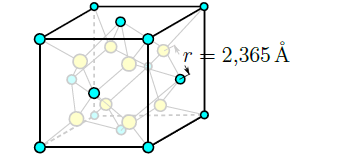
\includegraphics[scale=0.7]{Calciumflourid.png} \end{center}
\caption{Kristallstruktur von Kalziumflourid$^c$}
\end{figure}

\hrulefill\\
$^{a,b,c}$ Skriptum für das Praktikum zur Einführung in die Physikalische Chemie, Seite 2.

\vspace{10cm}
In den Bespielen liegt bei den ersten beiden Kristallen ein kubisch-flächenzentriertes Gitter und bei dem letzen Kristall ein kubisch-flächenzentriertes Gitter aus $\mathrm {Ca^{2+}-Ionen}$ und ein kubisch-primitives Gitter aus $ \mathrm {F^{-}-Ionen vor}$. Des weiteren gibt es etwa tetragonale, hexagonale, rhomboedrische sowie viele weitere Strukturen.\\ Eine primitive Elementarzelle enthält von jeder Atomart nur ein äquivalentes Atom. Die acht Atome in den Eckpunkten der Elementarzellen gehören nur zu einem achtel zu der Elementarzelle, da an jeder Ecke acht Elementarzellen aufeinander treffen.\\
In einer flächenzentrierten Elementarzelle befinden sich in den Ecken und in den Mitten aller sechs Flächen äquivalente Atome. Ein Atom auf einer Fläche gehört der Zelle zur Hälfte, eines auf der Kante zu einem viertel und eines im Zentrum der Zelle ganz.\\
Mithilfe dieser Informationen lässt sich berechnen, wie viele Formeleinheiten $N_{Z}$ auf eine Elementarzelle kommen. Beispielsweise kommt auf eine primitive Elementarzelle eine Formeleinheit, da wir acht Teilchen haben, die der Elementarzelle zu je einem achtel gehören.\\\\ Mithilfe folgender Überlegungen lässt sich die Masse $m_{Z}$ einer Elementarzelle bestimmen:

\begin{equation}
m_{Z}=Nz \cdot \dfrac{M}{N_{A}}
\end{equation} 

Das Volumen der Elementarzellen unserer zu untersuchender Kristalle lässt sich wie das Volumen eines Würfels folgendermaßen berechnen.

\begin{equation}
V_Z = a^3
\end{equation}


\subsection{Bestimmung der Loschmidt-Zahl}
 
Ziel des Versuchs ist es, die Loschmidt-Zahl $N_{A}$ durch den Vergleich von makroskopischer Dichte $p_{makro}$ mit mikroskopischer Dichte $p_{mikro}$ von exact geformten, zylindrischen Lithiumflourid-, Calciumflourid- und Aluminiumkristallen, zu bestimmen.\\\\

Die Makroskopische Dichte lässt sich durch  Masse und Volumen der Probekörper wie folgt errechnen:

\begin{equation}
p_{makro}= \frac{m_{Zyl}}{V_{Zyl}}
\end{equation}

Das Volumen des zylindrischen Probekörpers kann dabei durch genaue Bestimmung von Radius $r$ und Länge $l$ mithilfe folgender Formel bestimmt werden:

\begin{equation}
V_{zyl} = \pi \cdot r^{2} \cdot l
\end{equation}

Für die mikrospische Dichte $p_{mikro}$ einer Elementarzelle gilt, dass sie identisch zu der Makroskopischen Dichte ist, da ein Kristall durch die periodische Wiederholung seiner Elementarzellen aufgebaut ist.

\begin{equation}
p_{mikro}=\frac{m_Z}{V_Z}
\end{equation}

Masse und Volumen der Elementarzelle lassen sich mithilfe der oben aufgeführten Gleichungen 1 und 2 berechnen. Somit gilt unter Annahme, dass die makroskopische Dichte identisch zur mikroskopischen ist:

\begin{equation}
\frac{m_{Zyl}}{V_{Zyl}}= \frac{Nz \cdot M}{N_{A} \cdot a^3}
\end{equation}

Dies lässt sich nun nach $N_A$ umformen und wir erhalten folgende Frmel zur Berechnung der Loschmidt-Zahl:

\begin{equation}
N_A= \frac{N_Z \cdot M \cdot V_{Zyl}}{a^3 \cdot m_{Zyl}}
\end{equation}

\subsection{Bestimmung von $a$ des Kalciumflouridkristalls}
 
Um die Loschmidt-Zahl zu bestimmen wird der Wert $a$, die Kantenlänge einer Elementarzelle, benötigt. Dieser ist für die meisten Kristalle schon gegeben, lediglich für den Kalziumchlorid-Kristall muss sie noch ermittelt werden. Abbildung 3 zeigt die Kristallstruktur von Kalziumflourid. Es ist ein größeres kubisch-flächenzentriertes Gitter von $ \mathrm {Ca^{2+}}$-Ionen sowie ein darin liegendes, kleineres kubisch-primitives Gitter von $ \mathrm{F^-}$-Ionen erkennbar. Als Information ist uns der Abstand $r$ von den Ionen gegeben. Bei genauerer Betrachtung des Kristalls ist zu erkennen, dass ein Fluorid-Ion tetraedrisch von je vier Kalzium-Ionen umgeben ist. Der Abstand vom Zentrum zu den Ecken des Tetraeders entspricht dabei dem Abstand $r$.

\begin{figure} [h]
\begin{center}
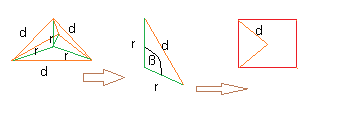
\includegraphics[scale=1]{a.png} \end{center}
\caption{Berechnung von $a$}
\end{figure} 

So lässt sich nun die Länge $d$ mithilfe des Kosinussatzes berechnen, da der Winkel in einem Tetraeder allgemein mit $109,5^\circ$ bekannt ist:

\begin{equation}
 d = \sqrt{2r^2-2r^2 \cdot \cos \beta } = 3, 863 \quad \AA
\end{equation}     

Die Länge $d$ ist die Hälfte der Flächen-diagonalen des Kalzium-Ionengitters. Da der Winkel zwischen den Flächen-diagonalen allgemein mit $ 90^\circ $ bekannt ist, lässt sich wieder mithilfe des Kosinussatzes die Länge $a$ berechnen:

\begin{equation}
 d = \sqrt{2d^2-2d^2 \cdot \cos \gamma } = 5,463 \quad \AA
\end{equation}   

\section{Experimentelles}

\subsection{Versuchsaufbau}
\subsection{Hilfsmittel}
Als Hilfsmittel werden eine Analysewaage sowie eine Mikrometerschraube verwendet.

\subsection{Durchführung}

Für die Bestimmung der Loschmidt-Zahl werden die drei Kristalle jeweils zehnmal gewogen und ausgemessen. Mithilfe der Analysewaage wird die Masse $m_{Zyl}$ bestimmt. Mit der Mikrometerschraube wird die Länge $l$ und Durchmesser $d$ gemessen. Im Umgang mit den Kristallen müssen Baumwollhandschuhe getragen werden. 

\section{Auswertung}
\section{Fehlerrechnung}
\section{Literaturverzeichnis}
1\quad Götz, Eckhold: \emph{Sriptum zur Einführung in die physikalische Chemie}, Institut für physikalische Chemie, Uni Göttingen, \textbf{2015}.

\vspace{0,5 cm}

2 \quad \emph{Skriptum für das Praktikum zur Einführung in die Physikalische Chemie}, Institut für physikalische Chemie, Uni Göttingen, \textbf{2015}.\\

3\quad Charles E. Mortimer, Ulrich Müller: \emph{Das Basiswissen der Chemie}, 7. Auflage, Georg Thieme Verlag, Stuttgart \textbf{2003}.


\end{document}